\documentclass[a4paper, 12pt]{article}
\usepackage[total={17cm,25cm}, top=2.5cm, left=2.5cm, right=2.5cm,  includefoot]{geometry}
\usepackage[utf8]{inputenc}
\usepackage{array}
\usepackage{multirow}
\usepackage{hhline}
\usepackage{gensymb}
\usepackage{graphicx}
\graphicspath{ {} }
\usepackage[czech]{babel}
\usepackage{enumitem}
\usepackage{pdfpages}
\usepackage{amsmath}
\usepackage{verbatim}
\usepackage{listings}
\usepackage{hyperref}
\usepackage{amssymb}


\pagestyle{empty} % vypne číslování stránek




\usepackage[OT2,OT1]{fontenc}
\newcommand\cyr
{
\renewcommand\rmdefault{wncyr}
\renewcommand\sfdefault{wncyss}
\renewcommand\encodingdefault{OT2}
\normalfont
\selectfont
}
\DeclareTextFontCommand{\textcyr}{\cyr}
\def\cprime{\char"7E }
\def\cdprime{\char"7F }
\def\eoborotnoye{\char’013}
\def\Eoborotnoye{\char’003}
\setlength{\parindent}{1em} 
%\setlength{\parskip}{0.5ex}


\begin{document}

\begin{titlepage}
\begin{center}
\Huge
\vspace*{4.5cm}
Algoritmy v digitální kartografii\\
\vspace{0.2cm}

\Large  
Digitální model terénu a jeho analýzy\\
\vspace{0.2cm}

\normalsize  
Zimní semestr 2018/2019\\
%(oprava: 24. 11. 2018)
\vspace{14cm}
\end{center}

\begin{flushright}
\Large
Tereza Kulovaná \\
Markéta Pecenová \\
\end{flushright}

\end{titlepage}


\pagestyle{plain}     % zapne obyčejné číslování
\setcounter{page}{1}  % nastaví čítač stránek znovu od jedné

\tableofcontents
\newpage

\section{Zadání}
Zadání úlohy bylo staženo ze stránek předmětu \href{https://web.natur.cuni.cz/~bayertom/index.php/teaching/algoritmy-v-digitalni-kartografii}{155ADKG}.

\begin{figure}[h!]
	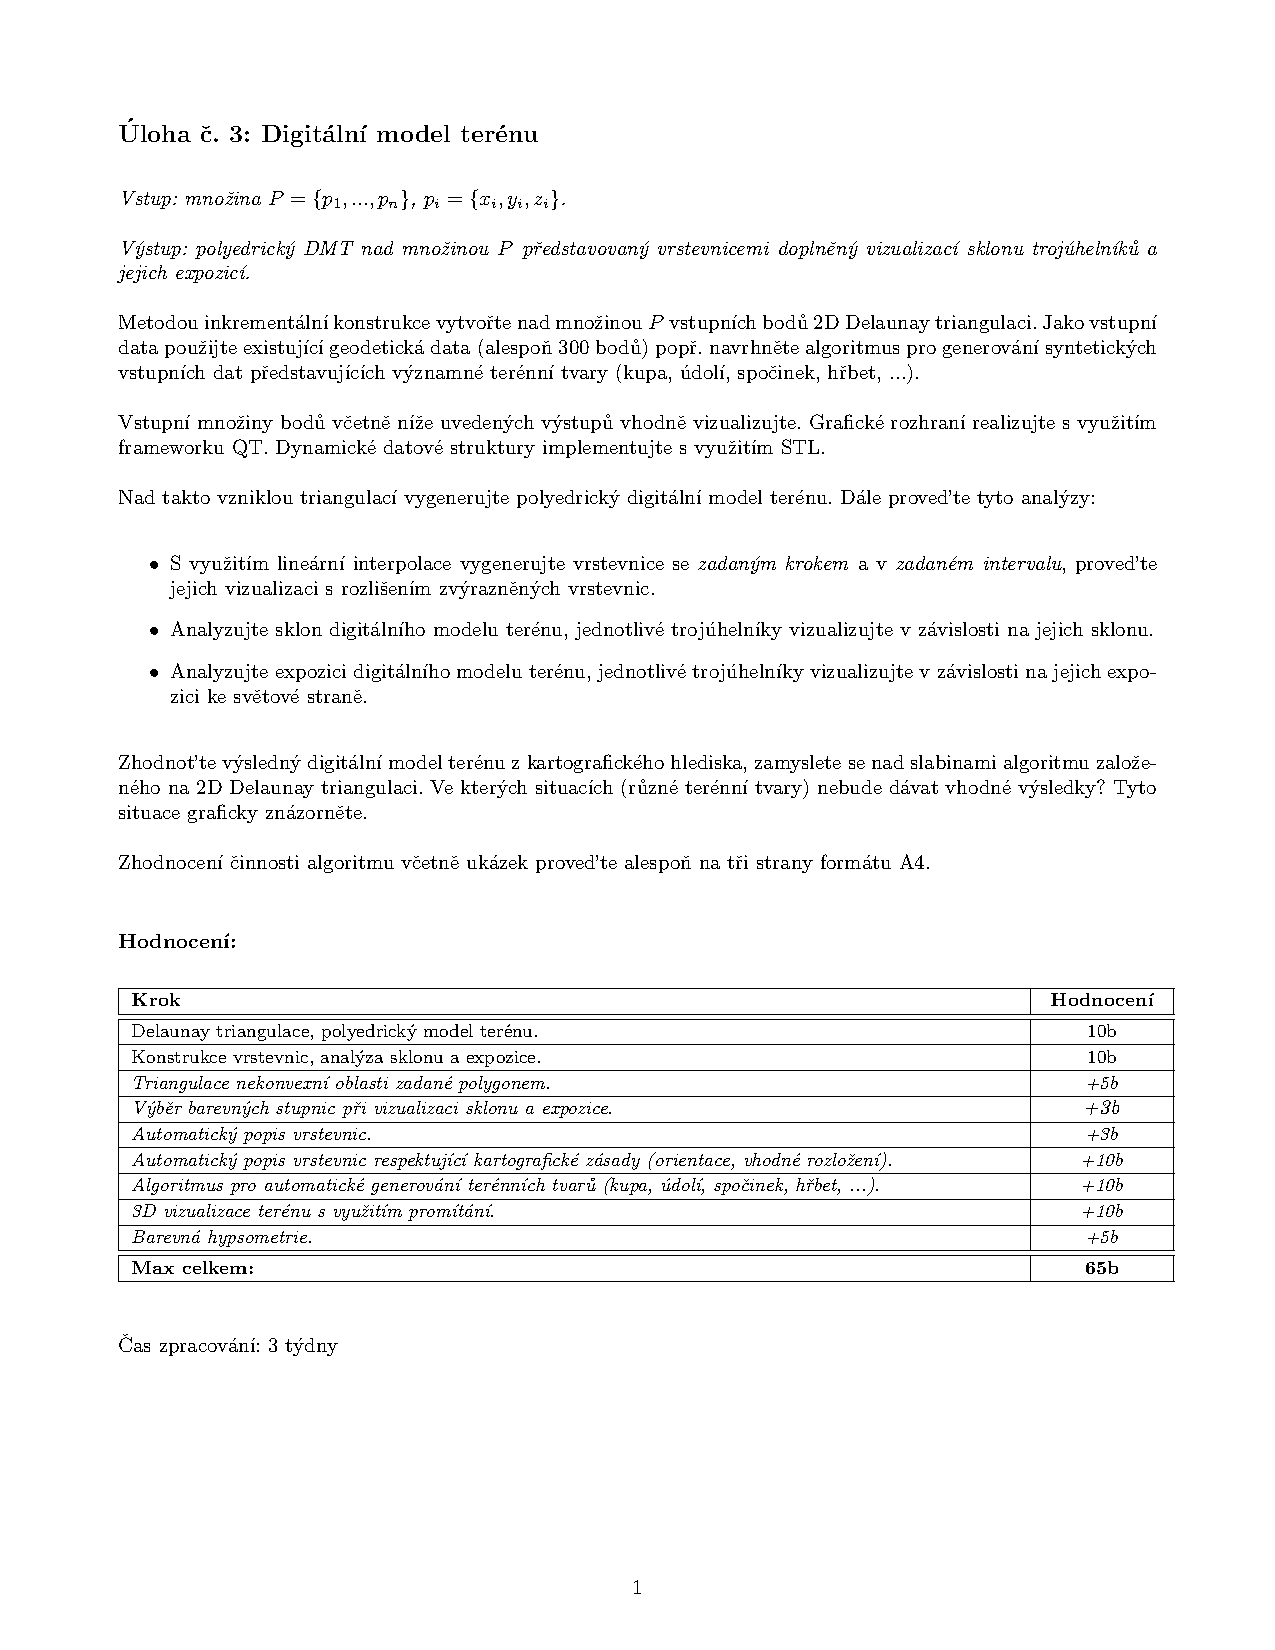
\includegraphics[clip, trim=0cm 4.5cm 0cm 3cm, width=1.0\textwidth]{./pictures/zadani03.pdf}
\end{figure}

V rámci této úlohy byly implementovány bonusové úlohy č. 
\clearpage

\section{Popis a rozbor problému}
Úloha \textbf{Digitální model terénu a jeho analýzy} se zabývá vytvořením aplikace, která Delaunayho triangulací vytvoří nad vstupní množinou bodů $P$ digitální model terénu. Dále  pro model lineární interpolací vypočte vrstevnice a sklon a expozici trojúhelníků ke světovým stranám. Vše je v aplikaci graficky zobrazeno.\\ 

Své využití konvexní obálky nalézají v mnoha oborech. V kartografii se hojně využívají při detekci tvarů a natočení budov pro tvorbu minimálních ohraničujících obdélníků. Dále jsou vhodné pro analýzu tvarů či shluků. Konvexní obálky lze sestrojit v libovolném $\mathbb{R}^n$ prostoru, avšak pro účely této úlohy byl uvažován pouze prostor $\mathbb{R}^2$. V rámci úlohy se testuje výpočetní rychlost použitých algoritmů při konstrukci obálek nad danými vstupními množinami bodů.

%\begin{figure}[h!]
	%\centering
	%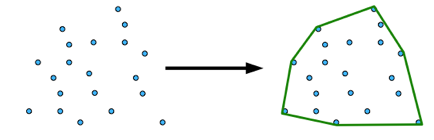
\includegraphics[width=13cm]{./pictures/ch.png}
	%\caption{Ukázka konvexní obálky (\href{http://mind.cs.byu.edu/courses/312/projects/project2_files/ConvexHull_python.php}{\textsl{zdroj}})}
%\end{figure}

Vzniklá aplikace k tvorbě konvexní obálek využívá tří výpočetních algoritmů: \textit{Jarvis Scan}, \textit{Quick Hull} a \textit{Sweep Line}.

\section{Algoritmy}
Tato kapitola se zabývá popisem algoritmů, které byly v aplikaci implementovány. 

\subsection{Jarvis Scan}
Prvním zvoleným algoritmem je \textit{Jarvis Scan}. Způsob, jakým vytváří konvexní obálku, nápadně připomíná balení dárků (proto je též občas nazýván jako \textit{Gift Wrapping Algorithm}). Mezi nevýhody tohoto algoritmu patří nutnost předzpracování dat a nalezení tzv. pivotu. Algoritmus dále není vhodný pro velké množiny bodů a ve vstupní množině $S$ nesmí být žádné tři body kolineární. Časová náročnost algoritmu je až $O(n^2)$, jeho výhodou však je velmi snadná implementace.\\

Mějme množinu bodů $S$ a pivota $q \in S$, jehož souřadnice Y je minimální ze všech bodů, a přidejme ho do konvexní obálky $H$. Následně do $H$ přidejme takový bod, který s posledními dvěma body přidanými do konvexní obálky svírá maximální úhel. Na začátku výpočtu je nutno inicializovat pomocný bod $s$, jehož souřadnice X je minimální a Y shodná s pivotem $q$, který zajistí dostatečný počet bodů pro výpočet prvního úhlu. Algoritmus končí ve chvíli, kdy nově přidaným bodem do konvexní obálky $H$ je opět pivot $q$. \\

Zjednodušený zápis algoritmu lze zapsat způsobem uvedeným níže:

\begin{enumerate}
\item Nalezení pivota $q$: $q$ = min($y$) 
\item Inicializace pomocného bodu $s$: $s$ = [min($x$), min($y$)]
\item Proveď: $q \in H$
\item Inicializace: $p_{j-1} = s$, $p_j = q$
\item opakuj kroky I–III, dokud $p_{j+1} \neq q$:
\begin{enumerate}[label=\Roman*.]
\item 	Najdi $p_{j+1}$: $\sphericalangle p_{j-1}, p_j, p_{j+1}$ = max
\item 	Proveď: $p_{j+1} \in H$
\item 	Přeindexuj: $p_{j-1} = p_j$, $p_j = p_{j+1}$
\end{enumerate}
\end{enumerate}

\subsection{Quick Hull}
Druhý algoritmus použitý v aplikaci je \textit{Quick Hull}, který k výpočtu konvexní obálky využívá strategii \textit{Divide and Conquer}. Hlavní výhodou algoritmu je jeho rychlost, která není ovlivňována velkým počtem rekurzivních kroků, jak tomu bývá u jiných algoritmů. Časová náročnost výpočtu bývá v nejhorším případě $O(n^2)$ a nastává tehdy, pokud všechny body množiny $S$ náleží konvexní obálce $H$.\\

Mějme body $q_1$, resp. $q_3$, jejichž souřadnice X je minimální, resp. maximální ze všech bodů z množiny $S$. Veďme těmito body pomyslnou přímku, která prostor rozdělí na horní ($S_U$) a dolní ($S_L$) polorovinu. Zbylé body množiny $S$ roztřídíme do daných polorovin podle jejich pozice od přímky. V polorovině následně hledáme bod, který je od dané přímky nejvzdálenější, přidáme ho do konvexní obálky dané poloroviny a přímkami spojíme bod s krajními body přímky předchozí. Proces opakujeme, dokud od nově vzniklých přímek již neexistují vhodné body. Na závěr do konvexní obálky $H$ přidáme bod $q_3$, body konvexní obálky $H_U$ z poloroviny $S_U$, bod $q_1$ a nakonec body konvexní obálky $H_L$ poloroviny $S_L$. Do konvexní obálky $H$ je důležité přidávat body v tomto pořadí, jinak by došlo k nesprávnému vykreslení konvexní obálky $H$. \\

Algoritmus \textit{Quick Hull} se skládá z globální a lokální procedury. Globální část zahrnuje rozdělení množiny na dvě poloroviny a spojení již nalezených bodů konvexních obálek polorovin do jediné $H$. V lokální části se rekurzivně volá metoda, která hledá nejvzdálenější body od přímky v dané polorovině a přidává je do konvexní obálky dané poloroviny $H_i$.\\

\textbf{Globální procedura}:
\begin{enumerate}
\item Inicializace: $H = \emptyset$, $S_U = \emptyset$, $S_L = \emptyset$ 
\item Nalezení $q_1$ = min($x$), $q_3$ = max($x$)
\item Proveď: $q_1 \in S_U$, $q_3 \in S_U$, $q_1 \in S_L$, $q_3 \in S_L$
\item Postupně pro všechna $p_i \in S$:
\subitem Podmínka ($p_i$ je vlevo od $q_1$, $q_3$) $\rightarrow S_U$
\subitem Jinak $ p_i \rightarrow S_L$
\item Proveď: $q_3 \in H$
\item Lokální procedura pro $S_U$
\item Proveď: $q_1 \in H$
\item Lokální procedura pro $S_L$
\end{enumerate}
~\\
\textbf{Lokální procedura nad polorovinou $S_i$}:
\begin{enumerate}[label=\Roman*.]
\item Pro všechny $p_i \in S_i$ kromě bodů přímky:
\subitem Podmínka ($p_i$ vpravo) $\rightarrow$ vzdálenost $d_i$
\subsubitem Podmínka ($d_i > d_{max}$) $\rightarrow d_{max} = d_i$, $p_{max} = p_i$
\item Podmínka (bod $p_{max}$ $\exists$) 
\subitem opakuj krok I. nad první nově vzniklou přímku
\subitem $p_{max} \in H_i$
\subitem opakuj krok I. nad druhou nově vzniklou přímku
\end{enumerate}

\subsection{Sweep Line}
Algoritmus \textit{Sweep Line} neboli \textit{Metoda zametací přímky} je dalším z algoritmů, které byly pro vytváření konvexních obálek implementovány. Jeho princip je založen na imaginární přímce, která se postupně přesouvá zleva doprava nad všemi body množiny $S$. Body, které \uv{přejede}, přidá do dočasné konvexní obálky \={H}, která je následně upravena, aby byla konvexní. Pro tento algoritmus je opět nutné předzpracování vstupních dat (seřadit body $\in S$ podle souřadnice X) s náročností $O(n.$log$(n))$. Další nevýhodou je citlivost algoritmu na singularity, konkrétně na duplicitní body. Ty je vhodné během předzpracování odstranit.\\ 

Algoritmus je postaven na znalosti pozice již vyhodnocených bodů vůči nově přidá\-vanému bodu ukládáním jejich indexů do proměnných $p$ (předchůdce) a $n$ (následník). Zároveň je pro správné fungování algoritmu nutné dodržovat CCW orientaci (proti směru hodinových ručiček). Algoritmus má celkem tři fáze: iniciální a dvě iterativní.\\

V první fázi seřadíme body $p_i$ z množiny $S$ vzestupně podle souřadnice X. Následně z prvních dvou bodů vytvoříme přímku, jejíž koncové body umístíme do konvexní obálky $H$ a indexy bodů umístíme do $n$ a $p$. V první iterativní fázi vyhodnotíme, zda další přidávaný bod leží v horní či dolní polorovině v závislosti na jeho souřadnici Y vzhledem k předchozímu bodu, a opět obousměrně vyhodnotíme indexy $n$ a $p$. Ve druhé iterativní fázi opravujeme dočasnou konvexní obálku \={H} na konvexní $H$ vložením horních a dolních tečen a vynecháním nekonvexních vrcholů.\\

Zjednodušený zápis algoritmu: 
\begin{enumerate}
\item Seřazení $p_i$ podle souřadnice X
\item Pro body $p_0$, $p_1$ proveď:
\subitem $n$[0] = 1, $n$[1] = 0
\subitem $p$[0] = 1, $p$[1] = 0
\item Pro všechna $p_i \in S$, $i > 1$ proveď:
\subitem Podmínka ($y_i > y_{i-1}$) $\rightarrow$ $S_U$: $p$[i] = i-1, $n$[i] = $n$[i-1]
\subitem Jinak $\rightarrow$ $S_L$: $n$[i] = i-1 $p$[i] = $p$[i-1]
\subitem Oprava indexů: $n$[$p$[i]] = i, $p$[$n$[i]] = i
\subitem Dokud $n$[$n$[i]] je vpravo od přímky (i, $n$[i]):
\subsubitem $p$[$n$[$n$[i]]] = i, $n$[i] = $n$[$n$[i]]
\subitem Dokud $p$[$p$[i]] je vlevo od přímky (i, $p$[i]):
\subsubitem $n$[$p$[$p$[i]]] = i, $p$[i] = $p$[$p$[i]]
\end{enumerate}

\section{Problematické situace}
V algoritmu \textit{Sweep Line} bylo nutné ošetřit singularitu, která způsobovala generování nekonvexní obálky. Konkrétně bylo nutné odstranit duplicitní body. V opravené verzi aplikace je situace ošetřena setříděním bodů podle souřadnice X a porovnáním vzdáleností mezi dvěma po sobě jdoucími body. Je-li vzdálenosti menší než stanovená mez $\epsilon$, body jsou považovány za duplicitní a bod s větší souřadnicí X je ze vstupní množiny odstraněn. \\

Podmínka ($d_{p_i,p_j} < \epsilon$) $\rightarrow$ bod $p_j$ nezahrnut (viz. Obrázek 2)\\


Algoritmus \textit{Jarvis Scan} generuje špatné výsledky, není-li ošetřeno, že žádné tři body nejsou spolu kolineární. Tento problém se zejména projevoval při generaci setu \textit{Grid}, který jich obsahuje spoustu. Singularita byla ošetřena vypočtením úhlu $\sphericalangle p_{jj}, p_j, p_i$, a pokud byl menší, než stanovená mez $\epsilon$, byl pro další výpočty vybrán bližší z kolineárních bodů.

\begin{itemize}
\item Podmínka ($\sphericalangle p_{jj}, p_j, p_i$) $< \epsilon$
\subitem Podmínka ($d_{p_j,p_i} < d_{min}$) $\rightarrow$ vyber bod $p_i$, $d_{min} = d_{p_j,p_i}$
\end{itemize}

Dalším problémem bylo, jak zajistit, aby byl generovaný rastr pravidelný. To bylo ošetřeno zaokrouhlením počtu vstupních bodů směrem nahoru tak, aby po odmocnění vznikl pravidelný rastr.\\

počet bodů v řádce/sloupci = $roundUp(\sqrt{num\_of\_points})$

\section{Vstupní data}
Aplikace si na základě ručního zadání vstupních parametrů uživatelem sama vygeneruje potřebná vstupní data. Z rozbalovací nabídky \textbf{Shape of set} uživatel volí prostorové uspořádání generované množiny bodů. Na výběr jsou možnosti \textit{Random set}, \textit{Grid} a \textit{Circle}. V kolonce \textbf{Number of points} uživatel volí, kolik bodů bude generováno. Lze tak učinit buď přímým zadáním počtu bodů, nebo zvýšením/snížením počtu bodů o 1000 šipkami na boku. Aplikace omezuje minimální a maximální počet generovaných bodů na interval $\textless$1, 1000000$\textgreater$. Množina bodů se vygeneruje stisknutím tlačítka \textsl{Generate set}.\\

Uživatel má dále možnost volit, jaký výpočetní algoritmus bude použit pro tvorbu konvexní obálky. Rozbalovací nabídka \textbf{Method} nabízí celkem tři výpočetní algoritmy: \textit{Jarvis Scan}, \textit{Quick Hull} a \textit{Sweep Line}. Konvexní obálka je generována stisknutím tlačítka \textsl{Create CH}. Pokud před spuštěním procesu nebyla vygenerována žádná vstupní množina bodů, uživatel je upozorněn chybovou hláškou. 

\section{Výstupní data}
Vygenerovaná množina bodů a její konvexní obálka je vykreslena v grafickém okně aplikace. Aplikace dále vypisuje časy [ms], jak dlouho trvalo generování množiny a jak dlouho nad danou množinou běžel výpočetní algoritmus.\\

V rámci testování byly nad množinami bodů \textit{Random set}, \textit{Grid} a \textit{Circle} postupně spuštěny všechny tři algoritmy. Pro každou množinu a algoritmus byla pro daný počet bodů $n = \{1000, 5000, 10000, 25000, 50000, 75000, 100000, 200000, 500000, 1000000\}$ aplikace spuš\-tě\-na 10x, aby bylo získáno dostatečné množství testovacích dat. Z každé testované množiny bylo tedy získáno celkem 300 testovacích dat. Data byla ukládána do textového souboru a následně zpracována v \textit{Excelu}.


\clearpage
\section{Aplikace}
V následují kapitole je představen vizuální vzhled vytvořené aplikace tak, jak ji vidí prostý uživatel.

%\begin{figure}[h!]
	%\centering
	%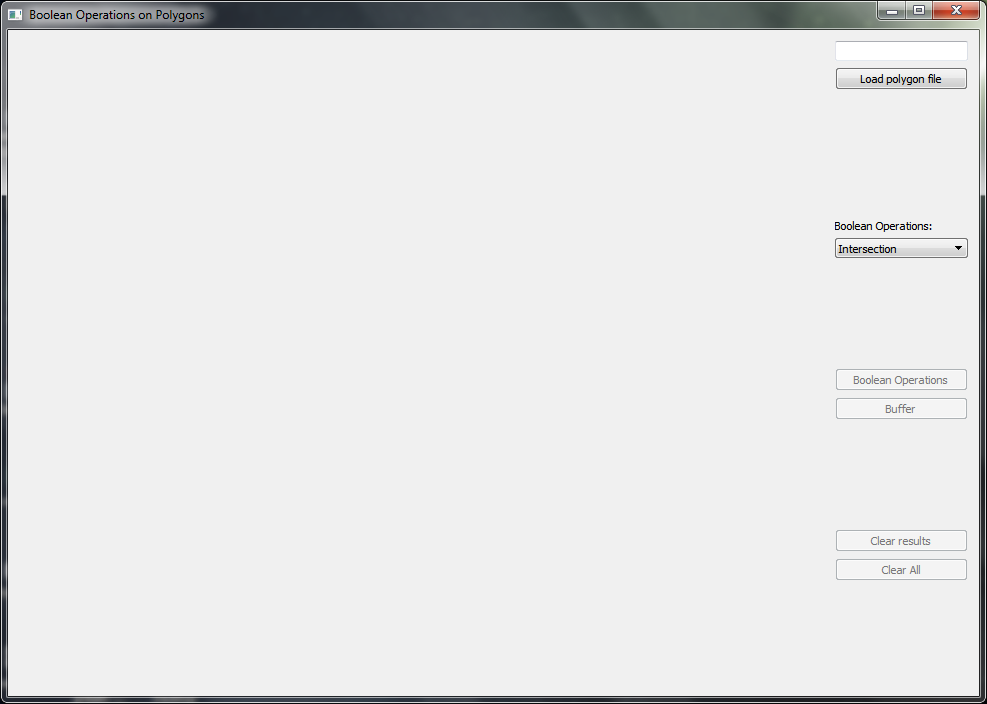
\includegraphics[width=11.5cm]{./pictures/app_default.png}
	%\caption{Výchozí vzhled aplikace po spuštění}
%\end{figure}



\clearpage
 
\section{Dokumentace}
Tato kapitola obsahuje dokumentaci k jednotlivým třídám.

\subsection{!Algorithms}
Třída \textit{Algorithms} obsahuje metody pro  které nad vstupní množinou bodů vytváří konvexní obálky. Dále obsahuje pomocné metody k výpočtu úhlu mezi dvěma přímkami, metody k určování vztahu bodu a přímky a metodu pro vytvoření striktně konvexní obálky.

\subsubsection*{delaunayTriangulation}
Metoda \textbf{delaunayTriangulation} vytváří nad množinou bodů Delaunayho triangulaci. Na vstupu je vektor bodů typu \texttt{QPoint3D}, metoda vrací uspořádaný vektor hran \texttt{Edge}, které tvoří jednotlivé trojúhelníky.\\

\textbf{Input}:
\begin{itemize}
\item \textsl{vector} $\textless$\texttt{QPoint3D}$\textgreater$ $points$
\end{itemize}

\textbf{Output}:
\begin{itemize}
\item \textsl{vector} $\textless$\texttt{Edge}$\textgreater$
\end{itemize}

\subsubsection*{!createContours}
Metoda \textbf{createContours} vytváří nad vstupní množinou hran vrstevnice na základě zadané minimální a maximální výšky a kroku, po kterém se vrstevnice budou vykreslovat.  Metoda vrací vektor hran, které představují vrstevnice.\\

\textbf{Input}:
\begin{itemize}
\item \textsl{vector} $\textless$\texttt{Edge}$\textgreater$ $dt$
\item \texttt{double} $z_min$ $\rightarrow$ minimální výška
\item \texttt{double} $z_max$ $\rightarrow$ maximální výška
\item \texttt{double} $dz$ $\rightarrow$ krok vrstevnic
\end{itemize}

\textbf{Output}:
\begin{itemize}
\item \textsl{vector} $\textless$\texttt{Edge}$\textgreater$
\end{itemize}

\subsubsection*{!getSlope}
Metoda \textbf{getSlope} počítá sklon trojúhelníku, který je tvořen třemi body. Návratová hodnota typu \texttt{double} nabývá hodnot $\textless$0$^\circ$;180$^\circ$???$\textgreater$ a vrací sklon trojúhelníku.\\

\textbf{Input}:
\begin{itemize}
\item \texttt{QPoint3D} $p_1$
\item \texttt{QPoint3D} $p_2$
\item \texttt{QPoint3D} $p_3$
\end{itemize}

\subsubsection*{!getAspect}
Metoda \textbf{getSlope} počítá orientaci trojúhelníku, který je tvořen třemi body, ke světovým stranám. Návratová hodnota typu \texttt{double} vrací orientaci trojúhelníku ve stupních. Hodnota 0$^\circ$ je umístěna na xxx, orientace je pravotočiná/levotočivá.\\

\textbf{Input}:
\begin{itemize}
\item \texttt{QPoint3D} $p_1$
\item \texttt{QPoint3D} $p_2$
\item \texttt{QPoint3D} $p_3$
\end{itemize}

\subsubsection*{analyzeDTM}
Metoda \textbf{analyzeDTM} vytváří z vektoru hran trojúhelníky a počítá pro ně sklon a orientaci. Vypočtené hodnoty ukládá do datového typu \texttt{Triangle}. Návratová hodnota metody je vektor trojúhelníků typu \texttt{Triangle}.\\

\textbf{Input}:
\begin{itemize}
\item \textsl{vector} $\textless$\texttt{Edge}$\textgreater$ $dt$
\end{itemize}

\textbf{Output}:
\begin{itemize}
\item \textsl{vector} $\textless$\texttt{Triangle}$\textgreater$
\end{itemize}

\subsubsection*{getPointLinePosition}
Metoda \textbf{getPointLinePosition} určuje polohu bodu $q$ vzhledem k přímce tvořené dvěma body. Na vstupu jsou 3 body typu \texttt{QPoint3D}, návratová hodnota je nově definovaný typ \texttt{TPosition}.\\

\textbf{Input}:
\begin{itemize}
\item \texttt{QPoint3D} $q$
\item \texttt{QPoint3D} $a$
\item \texttt{QPoint3D} $b$
\end{itemize}

\textbf{Output}:
\begin{itemize}
\item \texttt{LEFT} $\rightarrow$ bod se nachází vlevo od přímky
\item \texttt{RIGHT} $\rightarrow$ bod se nachází vpravo od přímky
\item \texttt{ON} $\rightarrow$ bod se nachází na přímce
\end{itemize}

\subsubsection*{!getCircleRadius}
Metoda \textbf{getCircleRadius} počítá poloměr kružnice, která je tvořena 3 body. Na vstupu jsou 3 body typu \texttt{QPoint3D}, návratová hodnota typu \texttt{double} vrací velikost poloměru kružnice.\\ 

\textbf{Input}:
\begin{itemize}
\item \texttt{QPoint3D} $p_1$ 
\item \texttt{QPoint3D} $p_2$ 
\item \texttt{QPoint3D} $p_3$
\item !!!\texttt{QPoint3D} $c$
\end{itemize}

\subsubsection*{getDistance}
Metoda \textbf{getDistance} počítá vzdálenost mezi dvěma body. Na vstupu jsou 2 body typu \texttt{QPoint3D}, návratová hodnota typu \texttt{double} vrací vzdálenost mezi dvěma body.\\ 

\textbf{Input}:
\begin{itemize}
\item \texttt{QPoint3D} $p_1$ 
\item \texttt{QPoint3D} $p_2$
\end{itemize}

\subsubsection*{getNearestPoint}
Metoda \textbf{getNearestPoint} slouží k nalezení nejbližšího bodu z množiny bodů vzhledem k danému bodu $p$. Na vstupu je daný bod $p$ a vektor bodů typu \texttt{QPoint3D}. Návratová hodnota typu \texttt{int} vrací index nejbližšího bodu.

\textbf{Input}:
\begin{itemize}
\item \texttt{QPoint3D} $p$ 
\item \textsl{vector} $\textless$\texttt{QPoint3D}$\textgreater$ $points$
\end{itemize}

\subsubsection*{getDelaunayPoint}
Metoda \textbf{getDelaunayPoint} slouží k nalezení třetího bodu trojúhelníku, který splňuje Delaunayho kritérium nejmenší opsané kružnice. Na vstupu jsou dva body typu \texttt{QPoint3D}, které představují orientovanou hranu, a vektor bodů typu \texttt{QPoint3D}. Návratová hodnota typu \texttt{int} vrací index hledaného bodu.\\

\textbf{Input}:
\begin{itemize}
\item \texttt{QPoint3D} $s$ $\rightarrow$ počáteční bod hrany
\item \texttt{QPoint3D} $e$ $\rightarrow$ koncový bod hrany
\item \textsl{vector} $\textless$\texttt{QPoint3D}$\textgreater$ $points$
\end{itemize}

\subsubsection*{getContourPoint}
Metoda \textbf{getContourPoint} počítá průsečík hrany trojúhelníku tvořené dvěma body typu \texttt{QPoint3D} s rovinou o dané výšce Z. Návratová hodnota je typu \texttt{QPoint3D}.\\

\textbf{Input}:
\begin{itemize}
\item \texttt{QPoint3D} $p_1$ 
\item \texttt{QPoint3D} $p_2$ 
\item \texttt{double} $z$ 
\end{itemize}

\subsection{!Draw}
Třída \textit{Draw} obsahuje metody, které nahrávají a vykreslují vstupní množinu bodů. Dále zajišťuje vykreslení a smazání všech operací, kterou jsou nad množinou prováděny.

\subsubsection*{paintEvent}
Metoda \textbf{paintEvent} vykresluje vstupní množinu bodů, Delaunayho triangulaci, vrstevnice a sklon a orientaci trojúhelníků.

\subsubsection*{clearDT}
Metoda \textbf{clearDT} slouží k vymazání všech vykreslených dat.

\subsubsection*{getPoints}
Metoda \textbf{getPoints} slouží k získání vektoru bodů z kreslící plochy. Metoda vrací vektor bodů typu \texttt{QPoint3D}.

\subsubsection*{getDT}
Metoda \textbf{getPoints} slouží k získání vektoru hran z kreslící plochy. Metoda vrací vektor hran typu \texttt{Edge}.

\subsubsection*{setDT}
Metoda \textbf{setDT} slouží k převedení Delaunayho triangulace do kreslícího okna.

\subsubsection*{setContours}
Metoda \textbf{setContours} slouží k převedení vrstevnic do kreslícího okna.

\subsubsection*{setDTM}
Metoda \textbf{setDTM} slouží k převedení digitálního modelů terénu do kreslícího okna.


\subsection{Edge}
Třída \textit{Edge} slouží k manipulaci s orientovanými hranami. Definuje dva body typu \texttt{QPoint3D} jako počáteční a koncový bod hrany.

\subsubsection*{getS}
Metoda \textbf{getS} slouží k získání počáteční body hrany. 

\subsubsection*{getE}
Metoda \textbf{getE} slouží k získání koncový body hrany. 

\subsubsection*{switchOrientation}
Metoda \textbf{switchOrientation} prohazuje orientaci hrany.  

\subsubsection*{????operator}


\subsection{QPpoint3D}
Třída \textbf{QPpoint3D} slouží k definování nového datového typu \texttt{QPoint3D}, který je odvozen od typu \texttt{QPointF} a který navíc obsahuje souřadnici Z.

\subsubsection*{getZ}
Metoda \textbf{getZ} slouží k získání souřadnice Z daného bodu.

\subsubsection*{setZ}
Metoda \textbf{setZ} slouží k nastavení souřadnice Z daného bodu. 


\subsection{SortByXAsc}
Třída \textbf{SortByXAsc} má na vstupu dva body typu \texttt{QPoint3D}, návratová hodnota je typu \texttt{bool}. Metoda vrací bod s nižší  souřadnicí X. Mají-li oba body shodnou souřadnici X, vrací bod s nižší souřadnicí Y.\\

\textbf{Input}:
\begin{itemize}
\item \texttt{QPoint3D} $p_1$
\item \texttt{QPoint3D} $p_2$
\end{itemize}

\textbf{Output}:
\begin{itemize}
\item 0 $\rightarrow$ bod $p_2$ má nižší $x$ souřadnici
\item 1 $\rightarrow$ bod $p_1$ má nižší $x$ souřadnici
\end{itemize}

\subsection{Triangle}
Třída \textbf{Triangle} slouží k definování nového datového typu \texttt{Triangle}, který v sobě uchovává informaci o třech bodech typu \texttt{QPoint3D}, které tvoří trojúhelník, a o sklonu a expozici trojúhelníku.

\subsubsection*{getPi}
Metoda \textbf{getSlope} slouží k získání bodu $P_i$ daného trojúhelníku. 

\subsubsection*{getSlope}
Metoda \textbf{getSlope} slouží k získání sklonu daného trojúhelníku. 

\subsubsection*{getAspect}
Metoda \textbf{getAspect} slouží k získání orientace daného trojúhelníku. 


\subsection{Widget}
Metody třídy \textbf{Widget} slouží pro práci uživatele s aplikací. Metody na vstupu nemají žádné parametry a návratové hodnoty jsou typu \texttt{void}.

\subsubsection*{on\_delaunay\_button\_clicked}
Metoda \textbf{on\_delaunay\_button\_clicked} nad vstupní množinou bodů zobrazí Delaunayho triangulaci. 

\subsubsection*{on\_clear\_button\_clicked}
Metoda \textbf{on\_clear\_button\_clicked} vrací aplikaci do výchozí polohy smazáním všeho, co bylo vykresleno. 

\subsubsection*{on\_contours\_button\_clicked}
Metoda \textbf{on\_contours\_button\_clicked} nad vygenerovanou trojúhelníkovou sítí z Delaunayho triangulace vykreslí vrstevnice. 

\subsubsection*{on\_dtm\_button\_clicked}
Metoda \textbf{on\_dtm\_button\_clicked} obarví trojúhelníky vygenerované Delaunayho triangulací v odstínech šedi podle hodnoty sklonu daného trojúhelníku.

\subsubsection*{!!!aspect}



\clearpage
\section{Závěr}
V rámci úlohy \textit{Konvexní obálky} byla vytvořena aplikace, která nad vstupní množinou bodů vytváří striktně konvexní obálky. V rámci testování, která trvalo dlouho do noci a použitým počítačům dala pořádně zabrat, byla shromážděna data průměrné doby výpočtu striktně konvexní obálky pro jednotlivé algoritmy. Z časových důvodů byly implementovány jen některé bonusové úlohy. Opravená verze aplikace lépe implementuje odstraňo\-vá\-ní duplicitních bodů v algoritmu \textit{Sweep Line}, což výrazně přispělo ke snížení doby běhu algoritmu. V závislosti na tom byly upraveny hodnoty v tabulkách a grafy z nich vycházející.\\

Po nově provedeném opravném testování považujeme za nejvhodnější algoritmus pro výpočet konvexní obálky algoritmus \textit{Sweep Line}, a to i přesto, že pro množinu \textit{Grid} byl o něco málo rychlejší algoritmus \textit{Quick Hull}. Jeho rychlost se projevila hlavně u množiny \textit{Circle} (striktně konvexní obálku nad milionem bodů generoval průměrně pod desetinu sekundy). Pro množiny \textit{Random} a \textit{Grid} lze považovat algoritmus \textit{Quick Hull} za srovnatelný s algoritmem \textit{Sweep Line} co se týče výpočetní doby. Jeho slabina se však projevila u množiny \textit{Circle}, jejíž prostorové uspořádání zaručuje, že všechny body náleží konvexní obálce. Tady \textit{Quick Hull} trochu zaváhal a výpočtení doba se prodloužila. Jako nevyhovujícím pro tvorbu konvexních obálek byl shledán algoritmus \textit{Jarvis Scan}. Výpočet obálky mu i na malých množinách trval o poznání déle než ostatním algoritmům, avšak překvapila nás rychlost, s jakou se vypořádal s kružnicí v porovnání s jinými množinami.\\

Závěrem by bylo vhodné podotknout, že data z testování nejsou 100\% spolehlivá. Již v průběhu testování bylo zaznamenáno, že doba výpočtu algoritmu velmi závisí na výkonu použitého počítače (rozdíl v rychlostech byl až dvojnásobný) a také na tom, zda jsou v době testování na počítači spuštěny jiné aplikace (např. prohlížeč) nebo se provádí jiné úkony (např. psaní technické zprávy). To může být jednou z příčin vzniku odchylek a nepřesností, které se v datech občas vyskytují. Pro zachování přibližně konzistentních podmínek při testování byly použity dva notebooky s podobným výkonem.\\

Do budoucna by jistě šla rozšířit nabídka generovaných množin bodů a naprogramovat celková automatizace testování. Aktuální verze kódu pro testování obsahovala pouze cyklus na 10 opakování téhož výpočtu. Dále by mohl být naprogramován další výpočetní algoritmus, \textit{Graham Scan}, na který již autorky neměly čas. Mezi pozitivní přínosy úlohy zajisté patří objevení způsobu hromadného exportu grafů z \textit{Excelu} do formátu *.png.

\clearpage

\section{Zdroje}
\begin{enumerate}
\item  \textsl{BAYER, Tomáš. 2D triangulace, DMT} [online][cit. 4. 12. 2018].\\
Dostupné z: \href{https://web.natur.cuni.cz/~bayertom/images/courses/Adk/adk5.pdf}{https://web.natur.cuni.cz}

%\item  \textsl{CS 312 - Convex Hull Project} [online][cit. 10. 11. 2018].\\
%Dostupné z: \href{http://mind.cs.byu.edu/courses/312/projects/project2_files/ConvexHull_python.php}{http://mind.cs.byu.edu}


\end{enumerate}
\end{document}

%getCircleRadius c
%smazat datové typy z popisu a dát je jen do input/output
%hodnota sklonu
%getAspect orientace